
\documentclass[residuals.tex]{subfiles}
\begin{document}
\section{Residual Plot}

The residual data of the simple linear regression model is the difference between the observed data of the dependent variable y and the fitted values $\hat{y}$.
 

% Problem
 
Plot the residual of the simple linear regression model of the data set faithful against the independent variable waiting.
 


% Solution
 
We apply the lm function to a formula that describes the variable eruptions by the variable waiting, and save the linear regression model in a new variable eruption.lm. Then we compute the residual with the \texttt{resid} function.
\newpage
 
\begin{framed}
\begin{verbatim}
> eruption.lm = lm(eruptions ~ waiting, data=faithful) 
> eruption.res = resid(eruption.lm) 
\end{verbatim}
\end{framed}

We now plot the residual against the observed values of the variable waiting. 
\begin{framed}
	\begin{verbatim}

> plot(faithful$waiting, eruption.res, 
+     ylab="Residuals", xlab="Waiting Time", 
+     main="Old Faithful Eruptions") 
> abline(0, 0)                  # the horizon 
\end{verbatim}
\end{framed}
\newpage
\begin{figure}[h!]
\centering
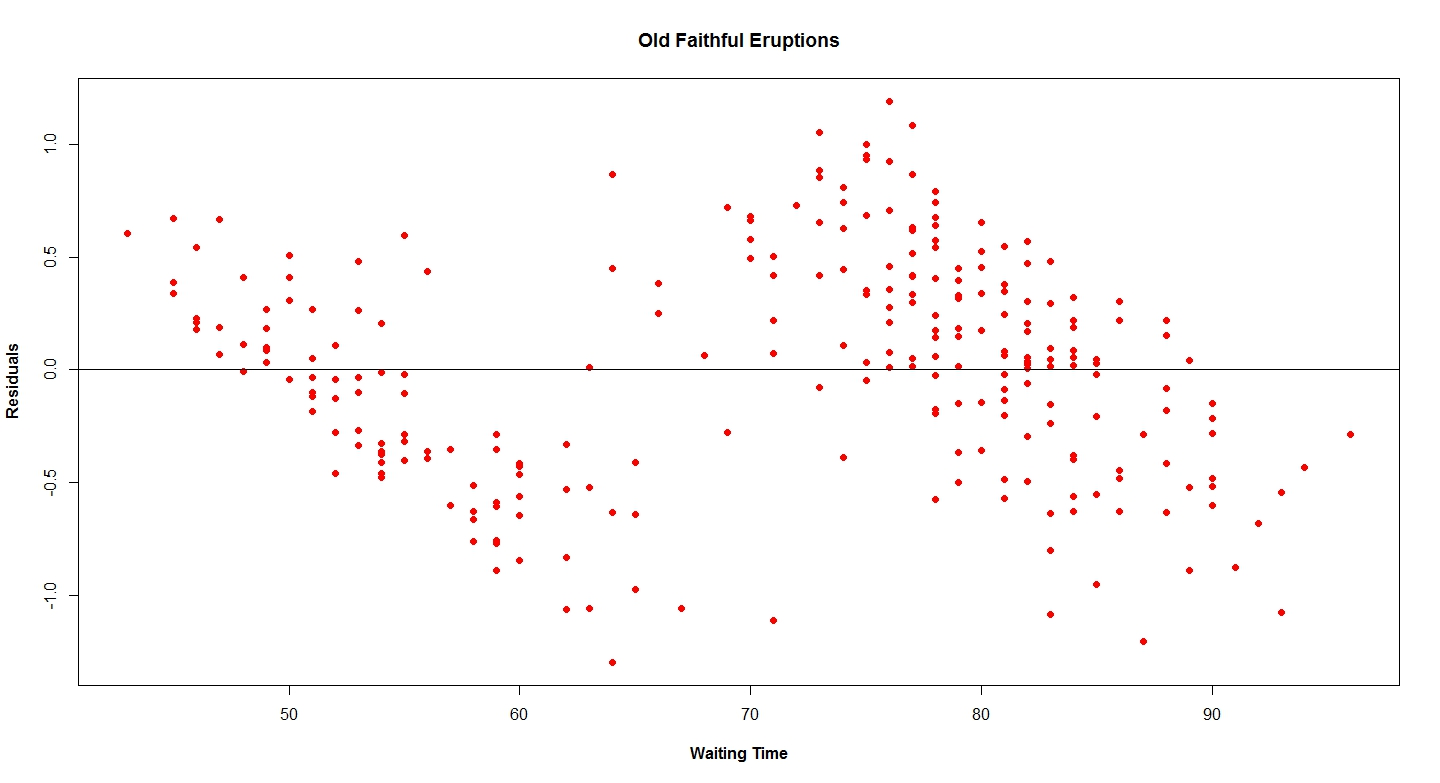
\includegraphics[width=0.99\linewidth]{oldfaithfulresiduals}
\caption{}
\label{fig:oldfaithfulresiduals}
\end{figure}

%=========================================================================================== %

\end{document}